\section{Results}\label{sec:results}

\begin{comment}
This section should detail the obtained results in a clear,
easy-to-follow manner. It is important to make clear what are original
results and what are repeats of previous calculations or computations.
Remember that long tables of numbers are just as boring to read as
they are to type-in!

Use graphs to present your results wherever practicable.

Results or computations should be presented with uncertainties
(errors), both statistical and systematic where applicable.

Be selective in what you include: half a dozen \emph{e.g.}~tables that
contain wrong data you collected while you forgot to switch on the
computer are not relevant and may mask the correct results.
\end{comment}

\subsection{Radar Data Fit}\label{subsec:radardatafit}

\begin{figure}[H]
    \centering
    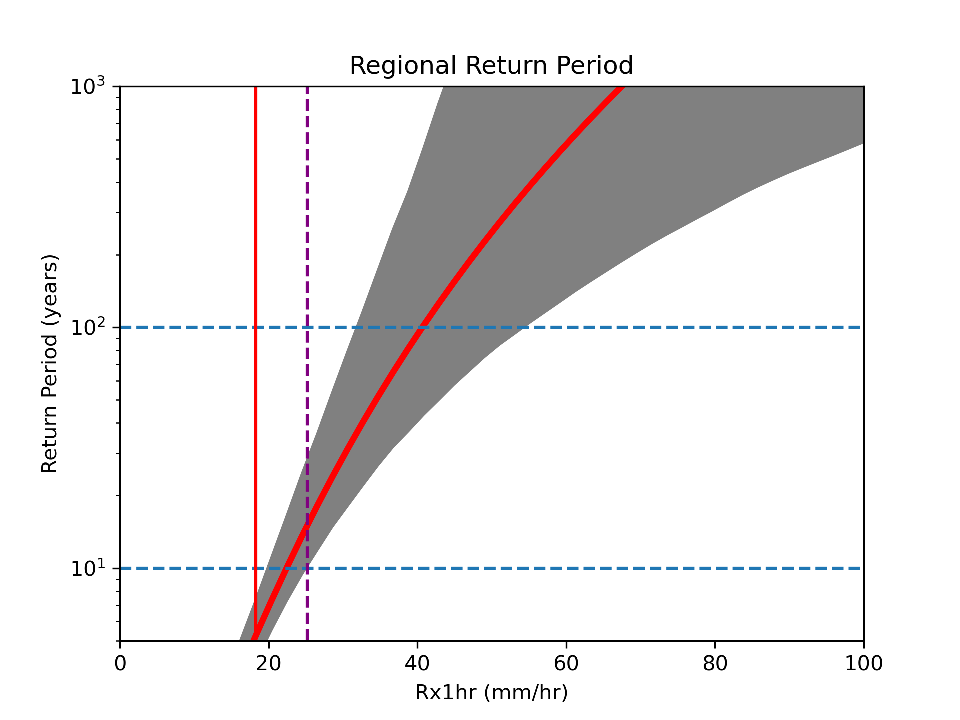
\includegraphics[width=150mm]{radarreturnplot}
    \caption{A line graph plotting the return period in years against the intensity of the event,
        taken from fitting a GEV distribution to the event distribution.
    The dashed purple vertical line is the intensity of the Stonehaven event.
    The solid red vertical line is the actual one-hour rainfall maximum at the Stonehaven crash location.
    The grey area gives the uncertainties from a Monte Carlo bootstrap of approximately 1000 samples.}
    \label{fig:radarreturnplot}
\end{figure}

It was found that the maximum hourly rainfall at the crash location was 18.2mm/hr and
    that the empirical return period for the Stonehaven event was 17 years,
    as can be seen in figure~\ref{fig:radarreturnplot}.
The intensity of the Stonehaven event,
    the 0.95 quantile of the radar grid cells having their 2020 seasonal maxima in the AM of the 12th of August,
    was found to be 25.2mm/hr.

Figure~\ref{fig:radarreturnplot} was created using the survival function of the GEV distribution fitted to the event data,
    getting the return period as the reciprocal of the probability.
This had parameters location $\mu = 10.7$, scale $\sigma = 4.26$ and shape $\xi = -0.173$.

\subsection{Model Data}\label{subsec:modelcorr}

\subsubsection{Model Correlations}

\begin{figure}[H]
    \centering
    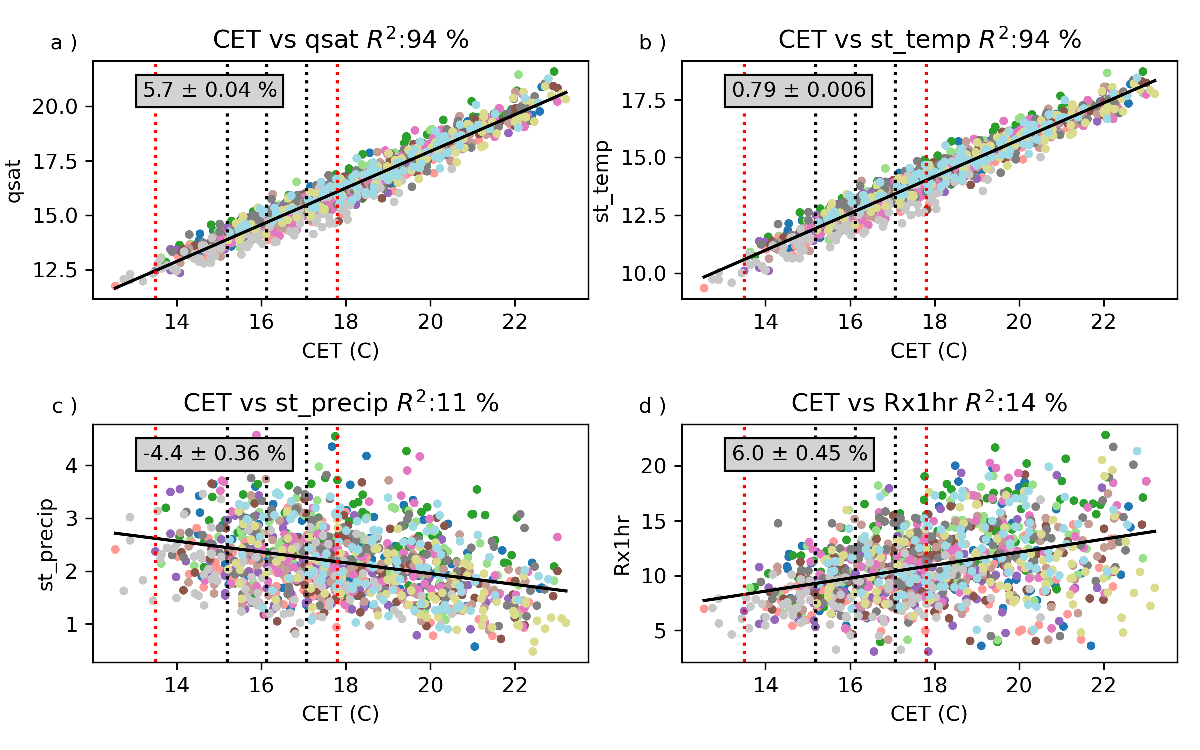
\includegraphics[width=150mm]{2cet_scatter}
    \caption{Scatter diagrams, from the Convection Permitting Model,
        for summer CET vs Stonehaven region saturated humidity (g/Kg) (a),
        Regional Temperature (b),
        Regional  Precipitation (mm/day) (c) and
        spatial median Rx1hr (mm/hr) for the region.
    The region is all points within a square of about 100x100km centered on the Stonehaven crash location.
    Colors indicate the ensemble number, black line is the best-fit regression slope.
    Text box shows best estimate and standard error in the estimated regression.
    Dotted black vertical lines show (left to right) CET summer mean for 1850--1899, 2021 and estimated CET at +2K warming.
    Title shows $R^2$ correlation coefficients for fit.
    Dotted vertical red lines show minimum and maximum CET values from 1850--2020 observations.}
    \label{fig:2cet_scatter}
\end{figure}

It is unsurprising that the correlations found in (a) and (b) are very similar,
    with both having $R^2$ values that round to the same number to the nearest percentage.
Some data points appear in almost identical points in both scatter diagrams.
This is evident from equation~\ref{eq:qsat}.
The by differentiating at $T=18$,
    equation~\ref{eq:qsat} has Taylor series to first order of $20.5627+1.2863(T-18)$.
By substituting $T=14$ and $T=22$ into this linear approximation,
    only small errors of $0.532$ and $0.603$ are found.
This suggests that in the CET range, equation~\ref{eq:qsat} is effectively linear and so the fit onto the Stonehaven Region saturated humidity
    is a linear scaling of the fit onto the Stonehaven Region Temperature.

\subsubsection{Model GEV fit}

\begin{figure}[H]
    \centering
    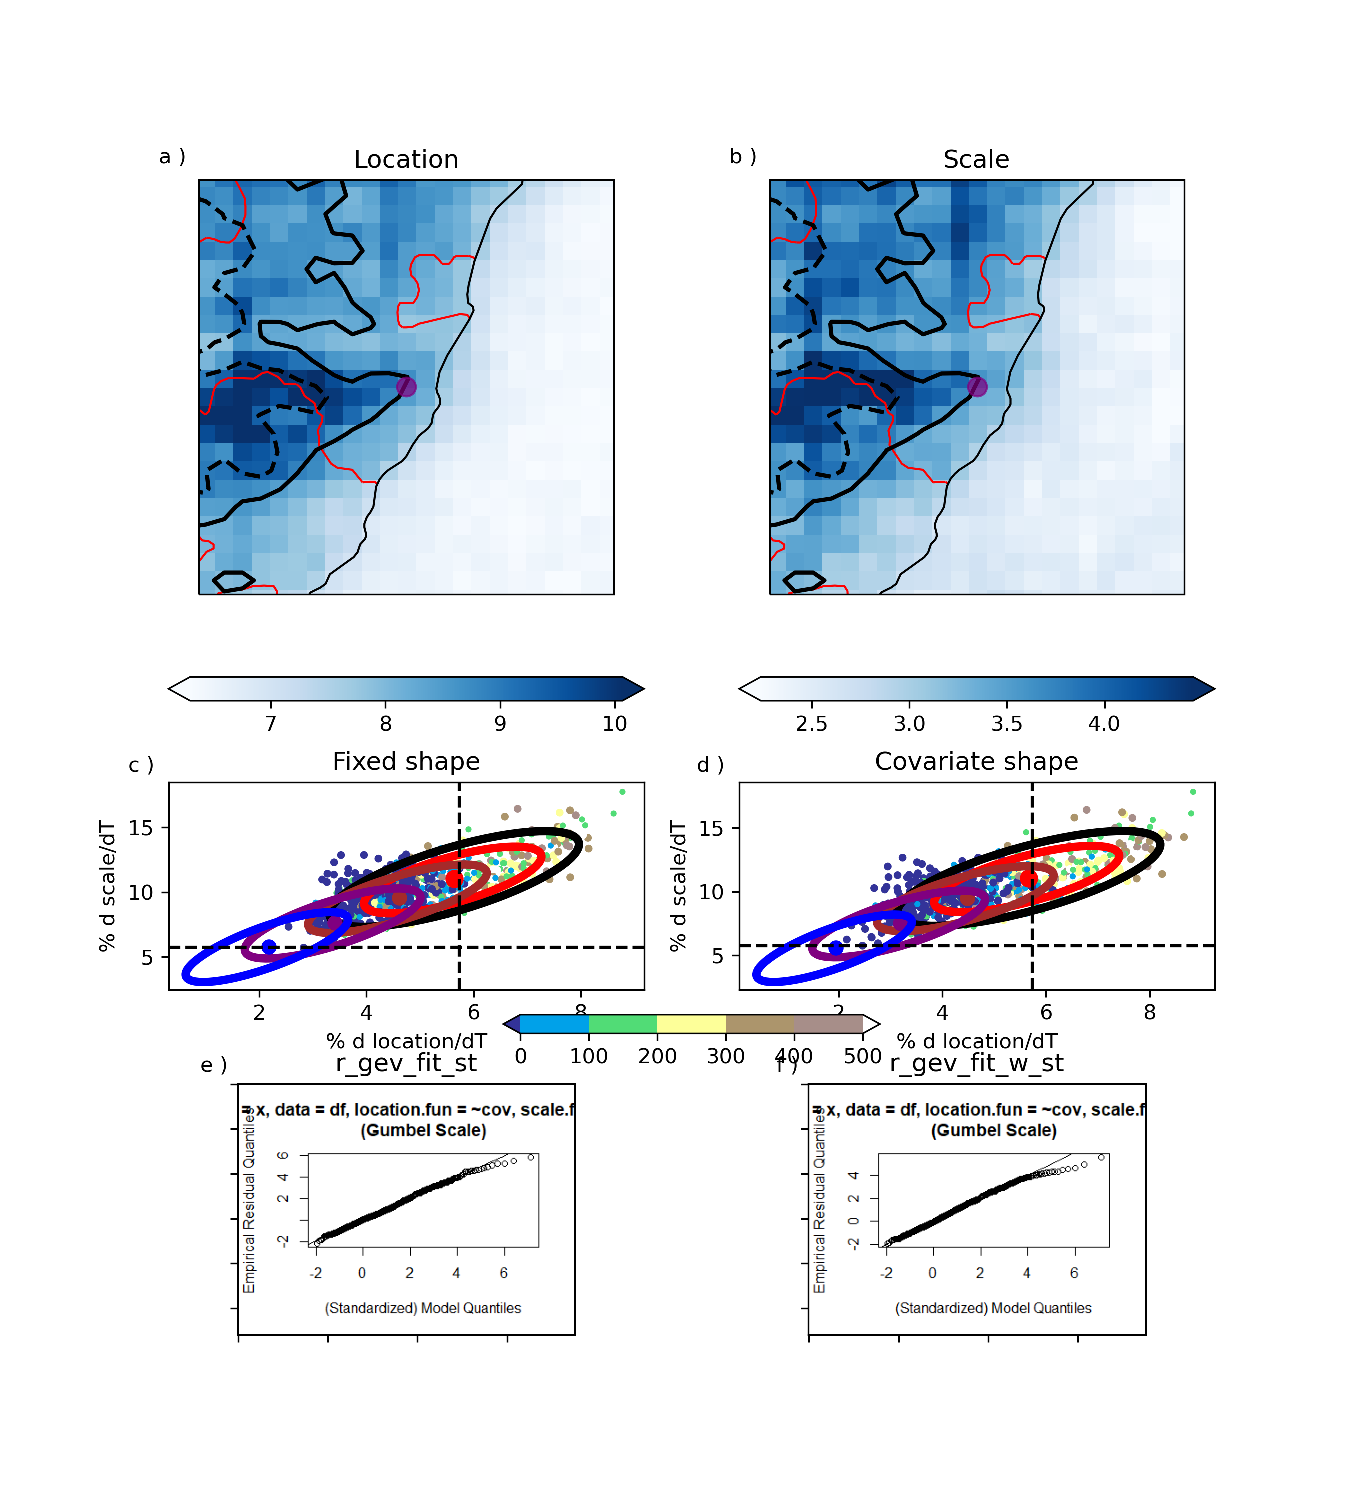
\includegraphics[width=100mm]{2cpm_gev_fit}
    \caption{a) Location parameter $\mu = \mu_0 + \overline{T_{2012-2021}}\mu_1$  for 2012--2021 CET and Rx1hr.
    b) Scale parameter $\sigma = \sigma_0 + \overline{T_{2012-2021}}\sigma_1$ for 2012--2021 CET and Rx1hr.
    c) Scatter plot of d(location)/d(CET) vs d(scale)/d(CET) as of 2012--2021 parameters.
    Dashed lines show expected changes if changes predicted by Clausius-Clapeyron relationship.
    Dots are colored by topography.
    Large red dot shows mean over all points where height is more than 0m and less than 400m.
    Red ellipse shows 95\% uncertainty for this mean, see subsection~\ref{subsec:riskratios}.
    Other colored large dots and ellipses show similar means and uncertainty ellipses for Rx2hr (brown), Rx4hr (purple) and Rx8hr (blue).
    Black ellipse shows 95\% uncertainty for all Rx1hr points where height is less than 0m and more than 200m.
    d) as c) but for case with shape parameter varying with CET
    e) QQ-plot for GEV fit to CPM data using CET as a covariate at the Stonehaven Crash location.
    f) as e) but for point 25km west of the Stonehaven Crash Location.}
    \label{fig:2cpm_gev_fit}
\end{figure}
\begin{table}[H]
    \centering
    \begin{tabular}{c c c c c}
        Covariate\textbackslash Data & Rx1h & Rx2h & Rx3h & Rx4h \\
        None &7498&6533&5341&4130 \\
        CET &7433&6482&5305&4109 \\
        CET w/ Shape &7434&6483&5305&4109 \\
        CPM Region &7402&6457&5287&4097 \\
        CPM Region w/ Shape &7403&6458&5287&4097 \\
        Stonehaven Region &7402&6457&5287&4098 \\
        Stonehaven Region w/ Shape &7403&6458&5288&4098 \\
        Stonehaven Humidity &7405&6459&5289&4099 \\
        Stonehaven Humidity w/ Shape &7406&6460&5290&4100 \\
    \end{tabular}
    \caption{AIC for maximum summer 1, 2, 4 and 8 hourly summer maximum rainfall
        above 0m and below 400m in the Stonehaven Region (+/- 0.5 degrees of the Stonehaven Crash location)
        GEV fits with different covariates.
    The covariates are CET, the average temperature in the CPM region (UK),
    the average temperature in the Stonehaven Region and
    the Saturation Humidity in the Stonehaven Region}
    \label{tab:AICtable}
\end{table}
\begin{table}[H]
    \centering
    \begin{tabular}{c c c}
        Dataset\textbackslash Parameter  & Location $\mu$ & Scale $\sigma$ \\
        Rx1hr &0.98&1.92 \\
        Rx2hr &0.80&1.67 \\
        Rx4hr &0.59&1.33 \\
        Rx8hr &0.38&1.01 \\
    \end{tabular}
    \caption{Ratio of mean parameter scalings to Clausius-Clapeyron scaling, $\left( \frac{\alpha_1}{\alpha_0} \right) / \left( \frac{H_1}{H_0} \right)$,
        for parameter $\alpha$ and saturated humidity $H$,
        where the shape parameter is fixed.
        Subscript $0$ is the value in the average summer CET of 2012--2021,
            subscript $1$ is the increase for every one degree increase of CET.
    Clausius-Clapeyron scaling is 5.73\%.}
    \label{tab:CCtable}
\end{table}


\subsection{Risk Ratios}\label{subsec:riskratio}

\begin{figure}[H]
    \centering
    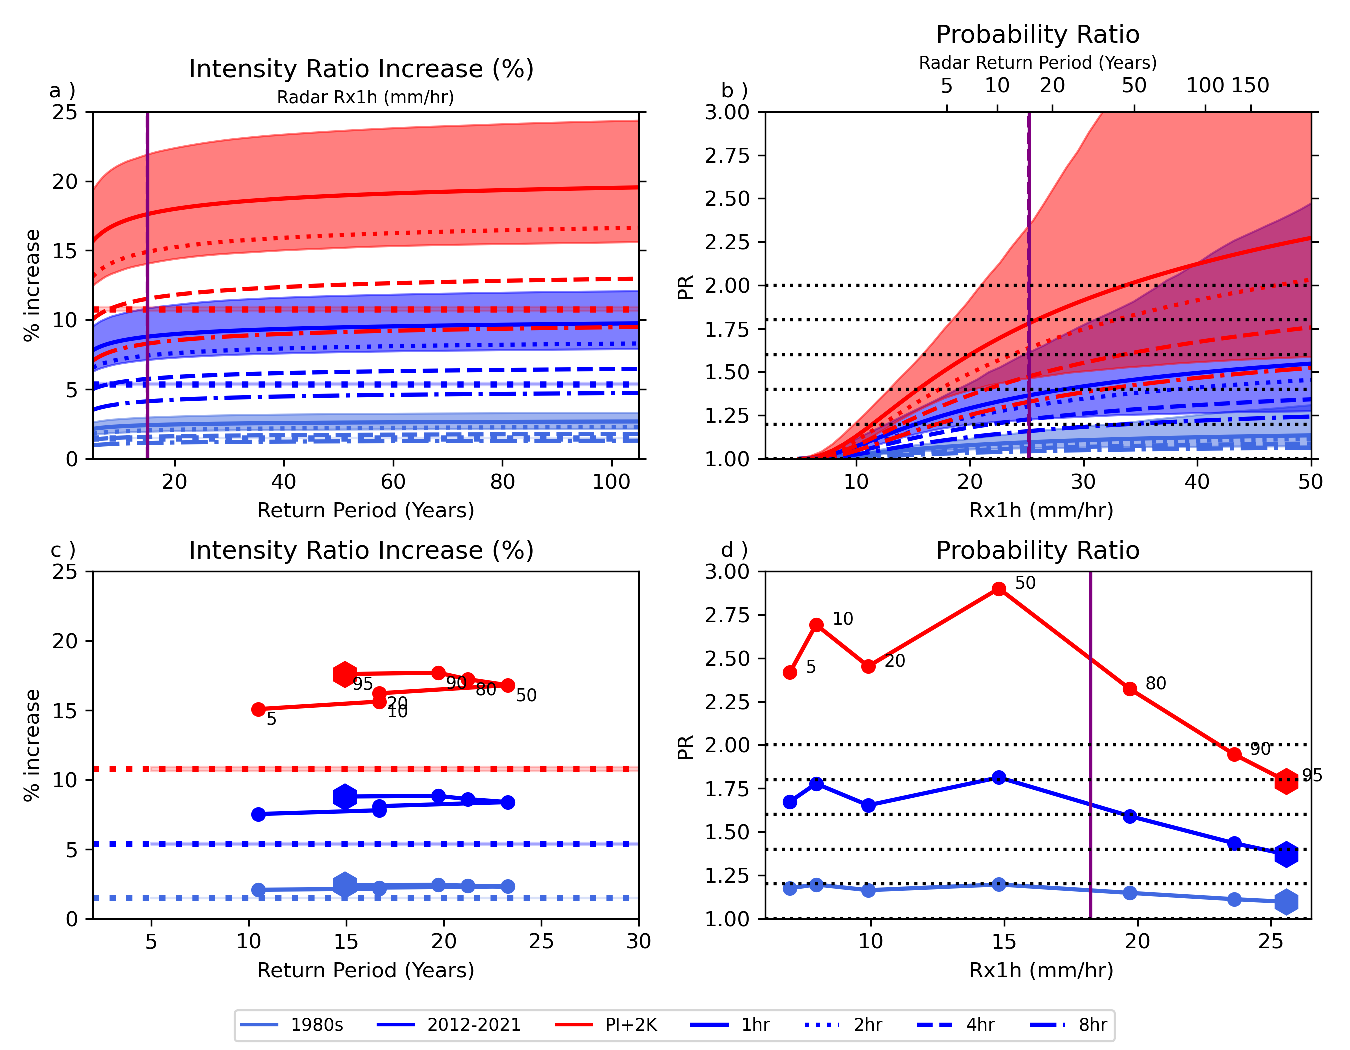
\includegraphics[width=\linewidth]{2probradarcpm}
    \caption{Intensity ratio increase (\%) as a function of the return period (a) and
    probability ratio as a function of regional Rx1hr (b).
    The best estimate (line) and 5--95\% uncertainty range (shading) are shown.
    Horizontal dotted lines in a) show expected intensity change if extremes scale with Clausius-Clapeyron.
    The top axis in a and b shows the equivalent rainfall and return period estimated from the radar rainfall data while
    vertical purple line shows the regional rainfall maximum for 2020.
    Dotted, dashed and dot-dashed lines in a and b show results when scaling estimated from simulated 2, 4 and 8 hourly summer maxima (Rx2hr, Rx4hr and Rx8hr).
    c) Intensity ratio increase (\%) as a function of return period for best estimates using different quantiles (labels on PI+2K line) to define regional extreme.
    Hexagon markers show 95\% quantile used in a and b.
    d) As c) but for probability ratio as a function of Rx1hr.
    Vertical purple line shows Stonehaven Crash Rx1hr for 2020-08-12.
    Note these are different from the regional 95\% quantiles shown in a and b.}
    \label{fig:2probradarcpm}
\end{figure}

\begin{figure}[H]
    \centering
    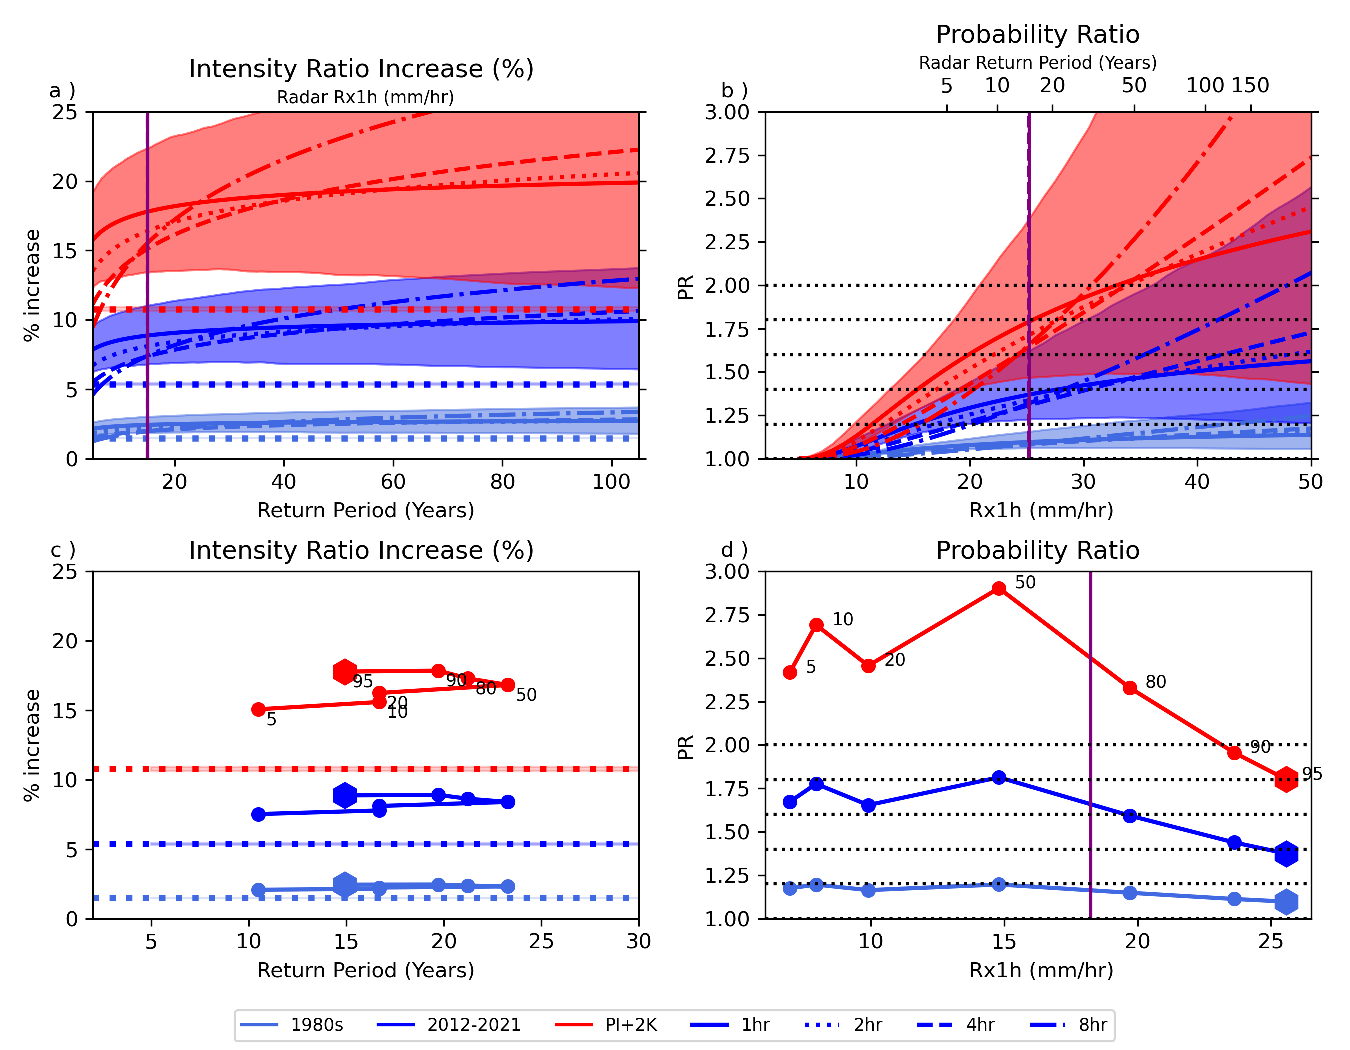
\includegraphics[width=\linewidth]{2probradarcpmshape}
    \caption{Identical to figure~\ref{fig:2probradarcpm},
    with the shape parameter also allowed to vary with CET.}
    \label{fig:2probradarcpmshape}
\end{figure}

\begin{table}[H]
   \centering
    \begin{tabular}{c c c}
        Time Period & Intensity Ratio (\%) & 5--95\% uncertainty (\%) \\
        1980s & 2 & 2--3 \\
        2012--2021 & 9 & 11--7 \\
        PI+2K & 18 & 14--22 \\
        With varying shape: && \\
        1980s & 2 & 2--3 \\
        2012--2021 & 9 & 11--7 \\
        PI+2K & 18 & 13--22 \\
    \end{tabular}
    \caption{A table with the intensity ratios $I_1/I_0$ for three different time periods,
        both with and without a covariate shape parameter.
    $I_1$ is the intensity of the event in the Time Period.
    $I_0$ is the intensity of the event Pre-Industrial (1850-1899).}
    \label{tab:irtable}
\end{table}

\begin{table}[H]
   \centering
    \begin{tabular}{c c c}
        Time Period & Probability Ratio (\%) & 5--95\% confidence interval (\%) \\
        1980s & 1.10 & 1.06--1.15 \\
        2012--2021 & 1.37 & 1.22--1.61 \\
        PI+2K & 1.78 & 1.46--2.34 \\
        With varying shape: && \\
        1980s & 1.10 & 1.06--1.15 \\
        2012--2021 & 1.37 & 1.23--1.62 \\
        PI+2K & 1.79 & 1.47--2.38 \\
    \end{tabular}
    \caption{A table with the probability ratios $p_1/p_0$ with confidence intervals for three different time periods,
        both with and without a covariate shape parameter.
    $p_1$ is the probability of the event in the Time Period.
    $p_0$ is the probability of the event Pre-Industrial (1850-1899).}
    \label{tab:prtable}
\end{table}

\begin{table}[H]
    \centering
    \begin{tabular}{c c c}
        Time Period\textbackslash Parameter & Location $\mu$ & Scale $\sigma$ \\
        PI & 10.2 & 3.90 \\
        1980s & 10.4 & 4.02 \\
        2012--2021 & 10.8 & 4.34 \\
        PI+2K & 11.3 & 4.79
    \end{tabular}
    \caption{A table showing the parameters of the GEV distribution for the intensity an event defined in subsection~\ref{subsec:radarprocess} after
        applying the scaling of the location $\mu$ and scale $\sigma$ parameters to the temperatures of different time periods.}
    \label{tab:0.95params}
\end{table}

The data in table~\ref{tab:0.95params} does not have a covariate shape,
    using the fixed shape parameter $\xi = -0.173$ from the empirical fit.
The shape parameter is in the $-0.174$--$-0.172$ range for all three fits with covariate shape,
    so it effectively duplicates the parameters here.

As the shape parameter is negative,
    it is possible to compute hypothetical the maximum,
    infinite return period intensity of an event using the formula $\mu - \frac{\sigma}{\xi}$.
This gives 32.7, 33.6, 35.9 and 39.0mm/hr as hypothetical maxima in
    PI, the 1980s, 2012--2021 and PI+2K Time Periods respectively.

\begin{figure}[H]
    \centering
    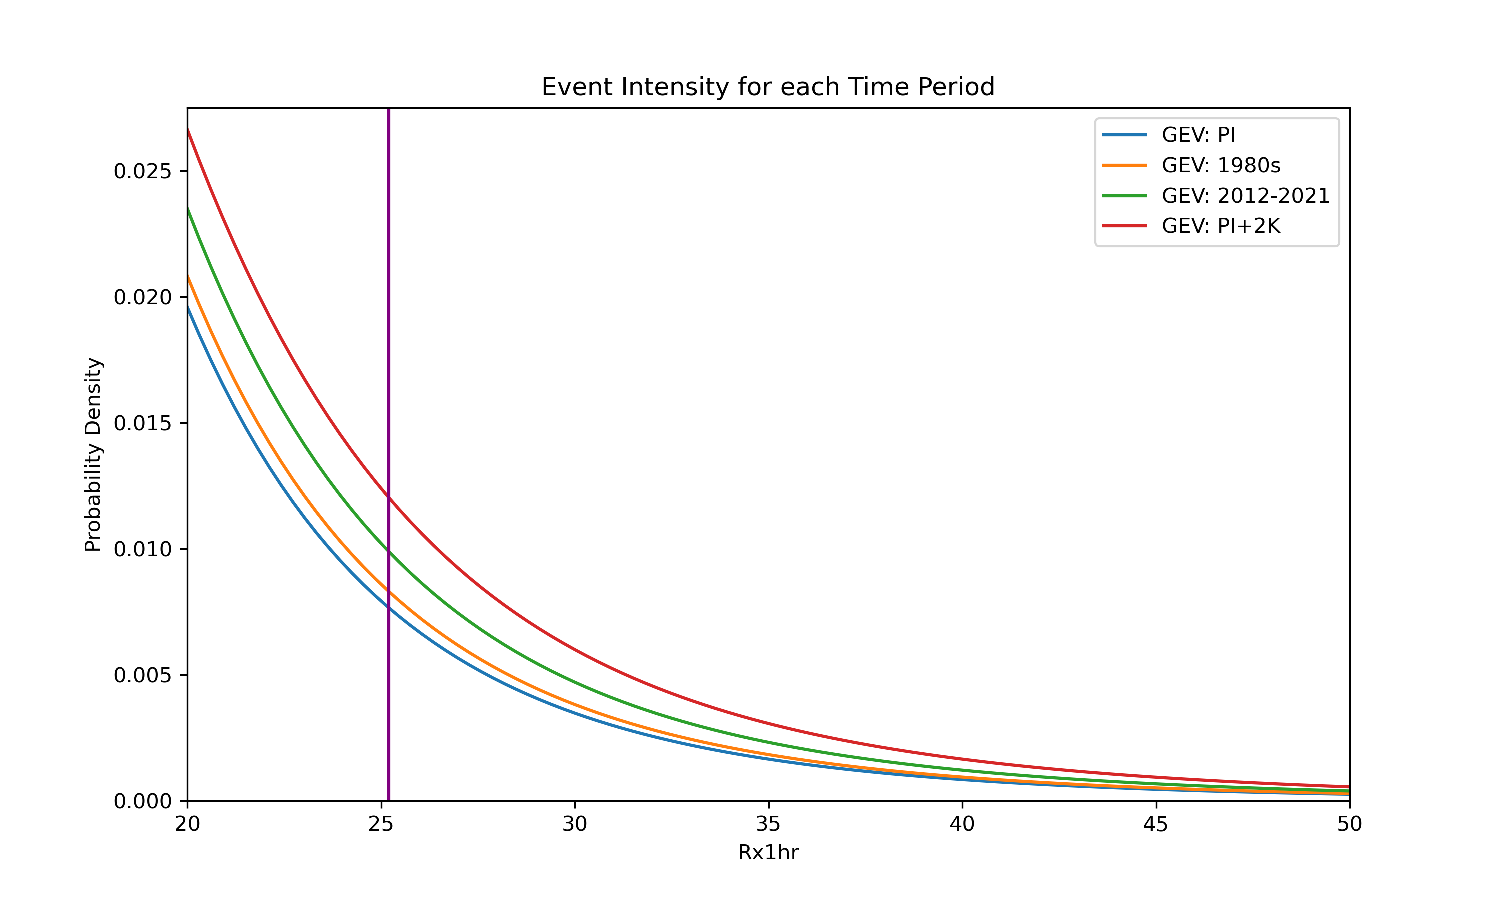
\includegraphics[width=150mm]{scaledgevdists}
    \caption{A line chart of the Probability Density Functions of the GEV distributions with parameters given in table~\ref{tab:0.95params},
        with a shape parameter $\xi = -0.172$.
    The Time periods are Pre-Industrial (PI), the 1980s, 2012-2021
    X-axis gives the 0.95 quantile of the maximum summer rainfall by grid cell,
        Y-axis gives the probability density in probability/Rx1hr.
    Vertical purple line is the intensity of the Stonehaven Event.}
    \label{fig:scaledgevdists}
\end{figure}

Figure~\ref{fig:scaledgevdists} illustrates the probability ratios in the top half of table~\ref{tab:prtable}.
$p_0$ is the area to the right of the purple line between 0 and the blue curve,
    while $p_1$ is the area to the right of the purple line between 0 and the yellow, green and red curves for
    the 1980s, 2012--2021 and a world 2K warmer than pre-industrial respectively.


\section{Discussion}\label{sec:discussion}

\begin{comment}
This section should give a picture of what you have taken out of your
project and how you can put it into context.

This section should summarise the results obtained, detail conclusions
reached, suggest future work, and changes that you would make if you
repeated the project.
\end{comment}

\subsection{Event Definition}\label{subsec:diseventdef}

%  TODO mention lack of trend analysis due to lack of radar data

%  TODO mention Koppen in analysis

\subsection{Model Resolution}\label{subsec:dismodeldef}

Mention~\cite{Kendon_Fischer_Short_2023}
%  TODO insert chart w various coarsenings

\subsection{Model Validity}\label{subsec:dismodelvalid}